% *********************************************************************
% © 2021 Jeremy Sylvestre
%
% Permission is granted to copy, distribute and/or modify this document
% under the terms of the GNU Free Documentation License, Version 1.3 or
% any later version published by the Free Software Foundation; with no
% Invariant Sections, no Front-Cover Texts, and no Back-Cover Texts. A
% copy of the license is included in the appendix entitled “GNU Free
% Documentation License” that appears in the output document of this
% PreTeXt source code. All trademarks™ are the registered® marks of
% their respective owners.
%
% *********************************************************************

\newcommand*{\xmin}{-0.1}
\newcommand*{\xmax}{0.8}
\newcommand*{\ymin}{-10}
\newcommand*{\ymax}{110}

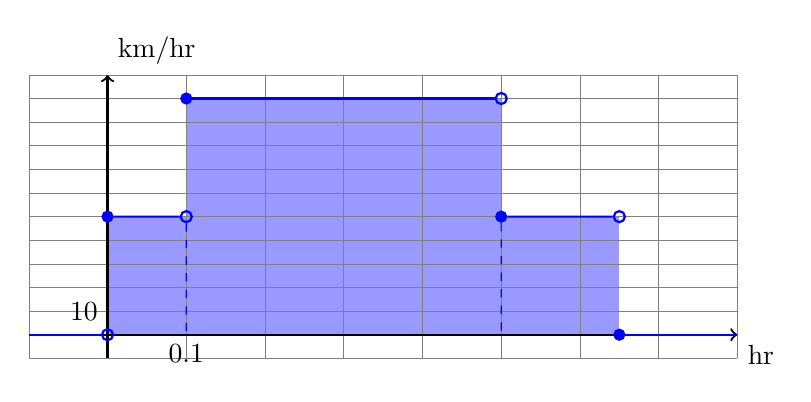
\begin{tikzpicture}
[
	closedpt/.style={circle,draw,fill,inner sep=0pt,minimum size=4pt},
	openpt/.style={circle,draw,inner sep=0pt,minimum size=4pt},
	xscale=10,
	yscale=0.03
]

	% rectangle fills
	\fill[blue!40!white] (0,50) rectangle (0.1,0);
	\fill[blue!40!white] (0.1,100) rectangle (0.5,0);
	\fill[blue!40!white] (0.5,50) rectangle (0.65,0);

	% grid
	\foreach \x in {-0.1,0.0,0.1,...,0.9} {   % I don't know why this needs to go past \xmax...
		\draw[very thin,gray] (\x,\ymin) -- (\x,\ymax);
	}
	\foreach \y in {-10,0,10,...,110} {
		\draw[very thin,gray] (\xmin,\y) -- (\xmax,\y);
	}

	% label grid
	\foreach \x in {0.1} {
		\node[below] at (\x,0) {$\x$};
	}
	\foreach \y in {10} {
		\node[left] at (0,\y) {$\y$};
	}

	% axes
	\draw[->,thick] (\xmin,0) -- (\xmax,0) node[below right] {hr};
	\draw[->,thick] (0,\ymin) -- (0,\ymax) node[above right] {$\mathrm{km}/\mathrm{hr}$};

	% before
	\node[blue,thick,openpt] at (0,0) (stop) {};
	\draw[blue,thick] (\xmin,0) -- (stop);

	% Camrose
	\node[blue,closedpt] at (0,50) (cstart) {};
	\node[blue,thick,openpt] at (0.1,50) (cstop) {};
	\draw[blue,thick] (cstart) -- (cstop);

	% highway
	\node[blue,closedpt] at (0.1,100) (hstart) {};
	\node[blue,thick,openpt] at (0.5,100) (hstop) {};
	\draw[blue,thick] (hstart) -- (hstop);

	% area divider
	\draw[blue,dashed]
	%   (hstart) -- (mstop)
	  (cstop) -- (0.1,0)
	;

	% Wetaskiwin
	\node[blue,closedpt] at (0.5,50) (wstart) {};
	\node[blue,thick,openpt] at (0.65,50) (wstop) {};
	\draw[blue,thick] (wstart) -- (wstop);

	% area divider
	\draw[blue,dashed]
	  (wstart) -- (0.5,0);
	;

	% off
	\node[blue,closedpt] at (0.65,0) (start) {};
	\draw[blue,thick] (start) -- (\xmax,0);

\end{tikzpicture}
